\documentclass{beamer}
%%%%%%%%%%%%%%%%%%%%%%%%%%%%%%%%%%%%%%%%%%%%%%%%%%%%%%%%%%%%%%%%%%%%%%%%%%%%%%%%%%%%%%%%%%%%%%%%%%
\setbeamertemplate{navigation symbols}{}
\usepackage{beamerthemeshadow}
\usefonttheme{serif}
%%%%%%%%%%%%%%%%%%%%%%%%%%%%%%%%%%%%%%%%%%%%%%%%%%%%%%%%%%%%%%%%%%%%%%%%%%%%%%%%%%%%%%%%%%%%%%%%%%
\usepackage{graphicx}
\graphicspath{ {res/} }
%%%%%%%%%%%%%%%%%%%%%%%%%%%%%%%%%%%%%%%%%%%%%%%%%%%%%%%%%%%%%%%%%%%%%%%%%%%%%%%%%%%%%%%%%%%%%%%%%%
\usepackage{polyglossia}
\setdefaultlanguage{armenian}
\setotherlanguages{english}
\usepackage{fontspec}
\newfontfamily\armenianfont{DejaVu Sans}
%%%%%%%%%%%%%%%%%%%%%%%%%%%%%%%%%%%%%%%%%%%%%%%%%%%%%%%%%%%%%%%%%%%%%%%%%%%%%%%%%%%%%%%%%%%%%%%%%%
\usepackage{minted}
\setminted[cpp]{fontsize=\footnotesize}
\setmonofont{Consolas}
%%%%%%%%%%%%%%%%%%%%%%%%%%%%%%%%%%%%%%%%%%%%%%%%%%%%%%%%%%%%%%%%%%%%%%%%%%%%%%%%%%%%%%%%%%%%%%%%%%
\usepackage{xltxtra}
\usepackage{hyperref}
%%%%%%%%%%%%%%%%%%%%%%%%%%%%%%%%%%%%%%%%%%%%%%%%%%%%%%%%%%%%%%%%%%%%%%%%%%%%%%%%%%%%%%%%%%%%%%%%%%
\usetheme{Luebeck}
\usecolortheme{crane}
%%%%%%%%%%%%%%%%%%%%%%%%%%%%%%%%%%%%%%%%%%%%%%%%%%%%%%%%%%%%%%%%%%%%%%%%%%%%%%%%%%%%%%%%%%%%%%%%%%
\definecolor{HTDark}{rgb}{0.04706, 0.13725, 0.26667} % primary color
\definecolor{HTLight}{rgb}{0.3686, 0.5255, 0.6235}   % secondary color
\setbeamercolor{palette primary}{bg=HTDark,fg=white}
\setbeamercolor{palette secondary}{bg=HTDark,fg=white}
\setbeamercolor{palette tertiary}{bg=HTDark,fg=white}
\setbeamercolor{palette quaternary}{bg=HTDark,fg=white}
\setbeamercolor{structure}{fg=HTDark} % itemize, enumerate, etc
\setbeamercolor{section in toc}{fg=HTDark} % TOC sections
\setbeamercolor{block title}{fg=white,bg=HTDark}
\setbeamercolor{block body}{fg=white, bg=HTLight}
\setbeamercolor{subsection in head/foot}{bg=HTLight,fg=white}
%%%%%%%%%%%%%%%%%%%%%%%%%%%%%%%%%%%%%%%%%%%%%%%%%%%%%%%%%%%%%%%%%%%%%%%%%%%%%%%%%%%%%%%%%%%%%%%%%%


\begin{document}

\title[Adapter]{Նախագծման Ձևանմուշներ։ Adapter}
\author[Հրաչյա Թանդիլյան\copyright]{Հրաչյա Թանդիլյան}
\date{2020}

%-------------------------------------------------------------------------------------------------
\begin{frame}
\titlepage
\end{frame}
%-------------------------------------------------------------------------------------------------

\section{Նպատակը}
%-------------------------------------------------------------------------------------------------
\begin{frame}\frametitle{Adapter}
\begin{block}{Նպատակը}
    Դասի ինտերֆեյսը փոխակերպում է օգտագործողի կողմից նախատեսված ինտերֆեյսի:
\end{block}
\vfill
Նաև հայտնի է որպես
\begin{itemize}
    \item Wrapper
\end{itemize}
\end{frame}
%-------------------------------------------------------------------------------------------------

\subsection{Մոտիվացիան}
%-------------------------------------------------------------------------------------------------
\begin{frame}\frametitle{Մոտիվացիան}
\begin{center}
    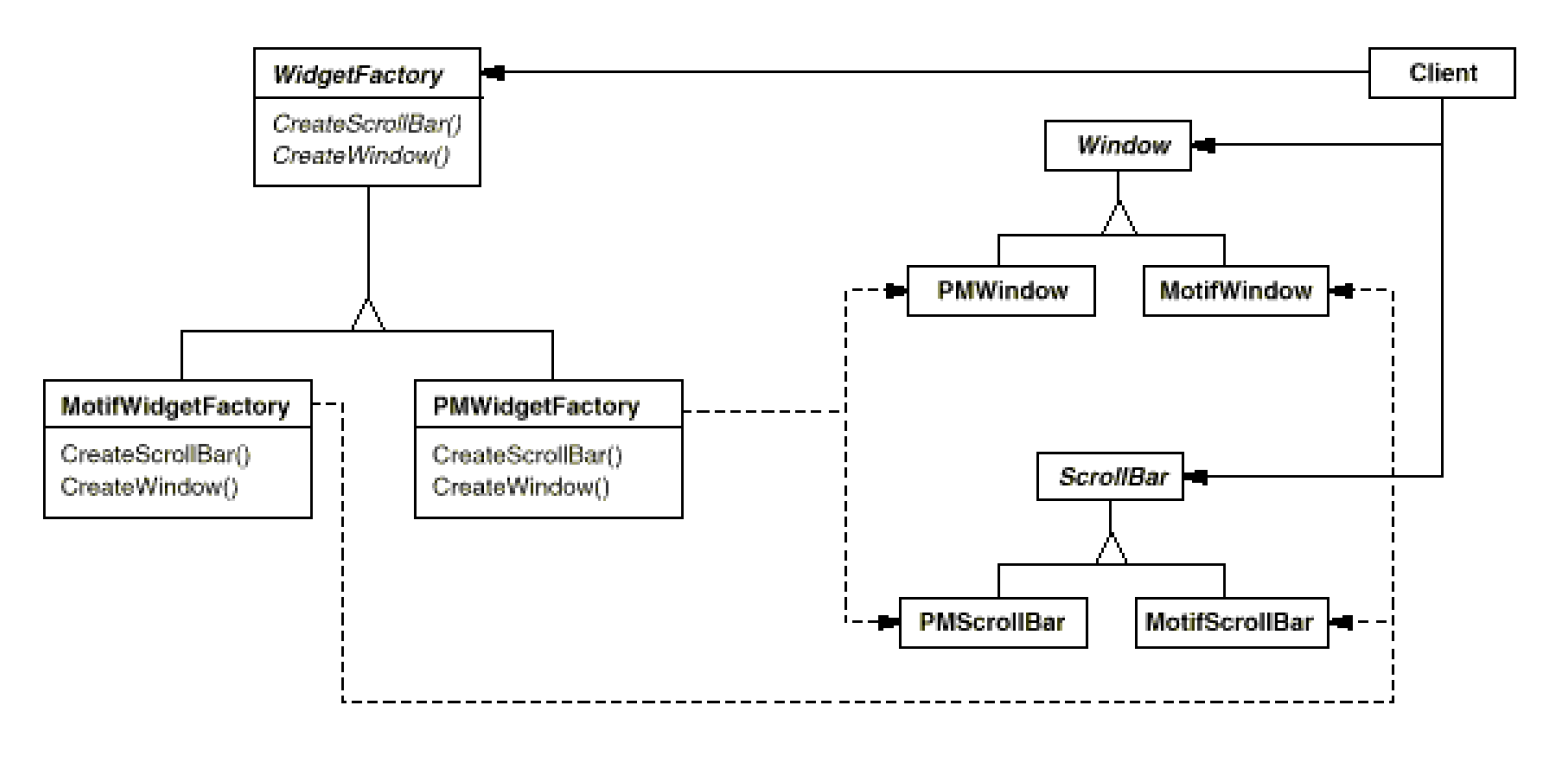
\includegraphics[scale=0.4]{motivation.png}
\end{center}
\end{frame}
%-------------------------------------------------------------------------------------------------

\subsection{Կիրառելիությունը}
%-------------------------------------------------------------------------------------------------
\begin{frame}\frametitle{Կիրառելիությունը}
Այս Ն.Ձ. պետք է օգտագործել երբ.
\vfill
\begin{enumerate}
    \item Ցանկանում եք օգտագործել գոյություն ունեցող դաս, բայց նրա ինտերֆեյսը չի
    համընկնում ձեզ անհրաժեշտ ինտերֆեյսի հետ: \pause \vfill
    \item Ցանկանում եք ստեղծել վերօգտագործելի դաս, որ կաշխատի չնախատեսված
    դասերի հետ, այսինքն այնպիսի դասերի հետ, որոնք պարտադիր չէ, որ ունենան
    պահանջվող ինտերֆեյսը \pause \vfill
    \item Միայն օբյեկտային Adapter-ի համար. ցանկանում եք օգտագործել մի շարք
    գոյություն ունեցող ենթադասեր, բայց նրանց ինտերֆեյսի փոխակերպում յուրաքանչյուրից
    ժառանգելու միջոցով պրակտիկ չէ:
\end{enumerate}
\end{frame}
%-------------------------------------------------------------------------------------------------

\section{Կառուցվածքը}
%-------------------------------------------------------------------------------------------------
\begin{frame}\frametitle{Կառուցվածքը: Class Adapter}
\begin{center}
    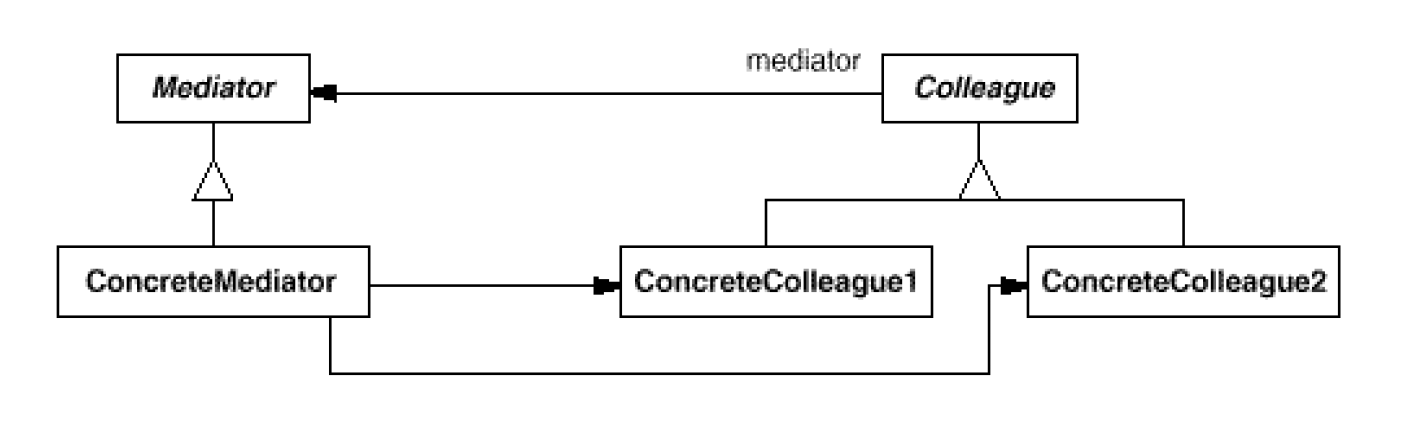
\includegraphics[scale=0.4]{structure1.png}
\end{center}
\end{frame}
%-------------------------------------------------------------------------------------------------

%-------------------------------------------------------------------------------------------------
\begin{frame}\frametitle{Կառուցվածքը: Object Adapter}
\begin{center}
    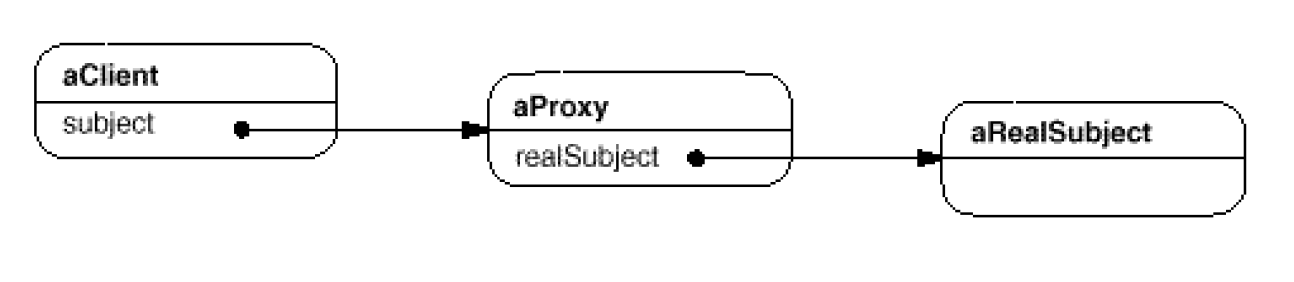
\includegraphics[scale=0.4]{structure2.png}
\end{center}
\end{frame}
%-------------------------------------------------------------------------------------------------

\subsection{Հետևանքները}
%-------------------------------------------------------------------------------------------------
\begin{frame}\frametitle{Հետևանքները: Class Adapter}
Այս Ն.Ձ. ունի հետևյալ առավելություններն ու թերությունները.
\vfill
\begin{enumerate}
    \item Փոխակերպում է կոնկրետ դասը և որպես հետևանք կիրառելի չէ երբ անհրաժեշտ է
    փոխակերպել դասը և նրա բոլոր ժառանգները: \vfill
    \item Թույլ է տալիս վերասահմանել ադապտացվող դասի որոշ վարվելակերպ, քանի որ
    հանդիսանում է նրա ժառանգը: \vfill
    \item Օգտագործում է միայն մեկ օբյեկտ, բացառելով հավելյալ վերահղման անհրաժեշտությունը:
\end{enumerate}
\end{frame}
%-------------------------------------------------------------------------------------------------

%-------------------------------------------------------------------------------------------------
\begin{frame}\frametitle{Հետևանքները: Object Adapter}
Այս Ն.Ձ. ունի հետևյալ առավելություններն ու թերությունները.
\vfill
\begin{enumerate}
    \item Թույլ է տալիս միակ Adapter-ին աշխատել շատ ադապտացվող դասերի հետ,
    այսինքն ադապտացվող դասի և նրա բոլոր ժառանգերի հետ: \vfill
    \item Դժվարեցնում է ադապտացվող դասի վարվելակերպի վերասահմանումը:
\end{enumerate}
\end{frame}
%-------------------------------------------------------------------------------------------------

%-------------------------------------------------------------------------------------------------
\begin{frame}\frametitle{Հետևանքները}
Այս Ն.Ձ. ունի նաև հետևյալ դիտարկման արժանի հարցերը.
\vfill
\begin{enumerate}
    \item Որքան փոխակերպում է Adapter-ը իրականացնումը: \vfill
    \item Pluggable adapter-ներ: \vfill
    \item Թափանցիկության համար երկակի Adapter-ների կիրառում:
\end{enumerate}
\end{frame}
%-------------------------------------------------------------------------------------------------

\section{Իրականացումը}
%-------------------------------------------------------------------------------------------------
\begin{frame}\frametitle{Իրականացումը}
\begin{enumerate}
    \item Class adapter-ի իրականացումը C++ \vfill
    \item Pluggable adapter-ներ: \vfill
    \begin{itemize}
        \item Աբստրակտ մեթոդների կիրառմամբ: \vfill
        \item Ներկայացուցիչ (delegate) օբյեկտների կիրառմամբ:
    \end{itemize}
\end{enumerate}
\end{frame}
%-------------------------------------------------------------------------------------------------

%-------------------------------------------------------------------------------------------------
\begin{frame}\frametitle{Pluggable Adapter-ների Իրականացումը}
Աբստրակտ մեթոդների կիրառմամբ: \vfill
\begin{center}
    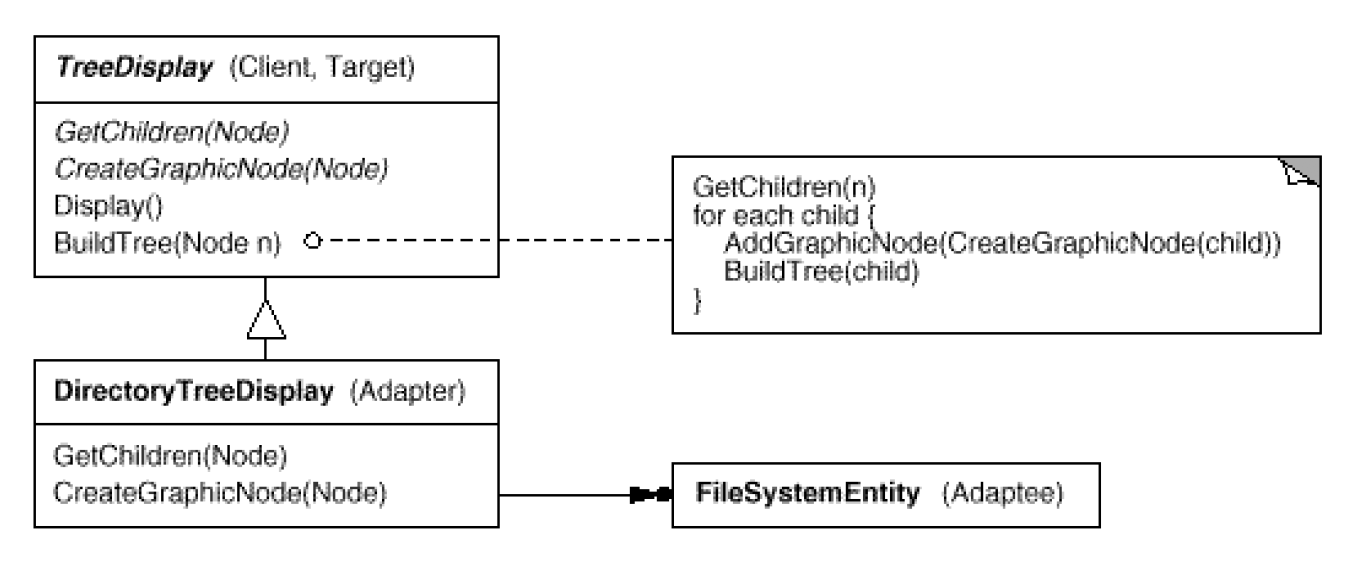
\includegraphics[scale=0.4]{pluggableadapter1.png}
\end{center}
\end{frame}
%-------------------------------------------------------------------------------------------------

%-------------------------------------------------------------------------------------------------
\begin{frame}\frametitle{Pluggable Adapter-ների Իրականացումը}
Ներկայացուցիչ օբյեկտների կիրառմամբ: \vfill
\begin{center}
    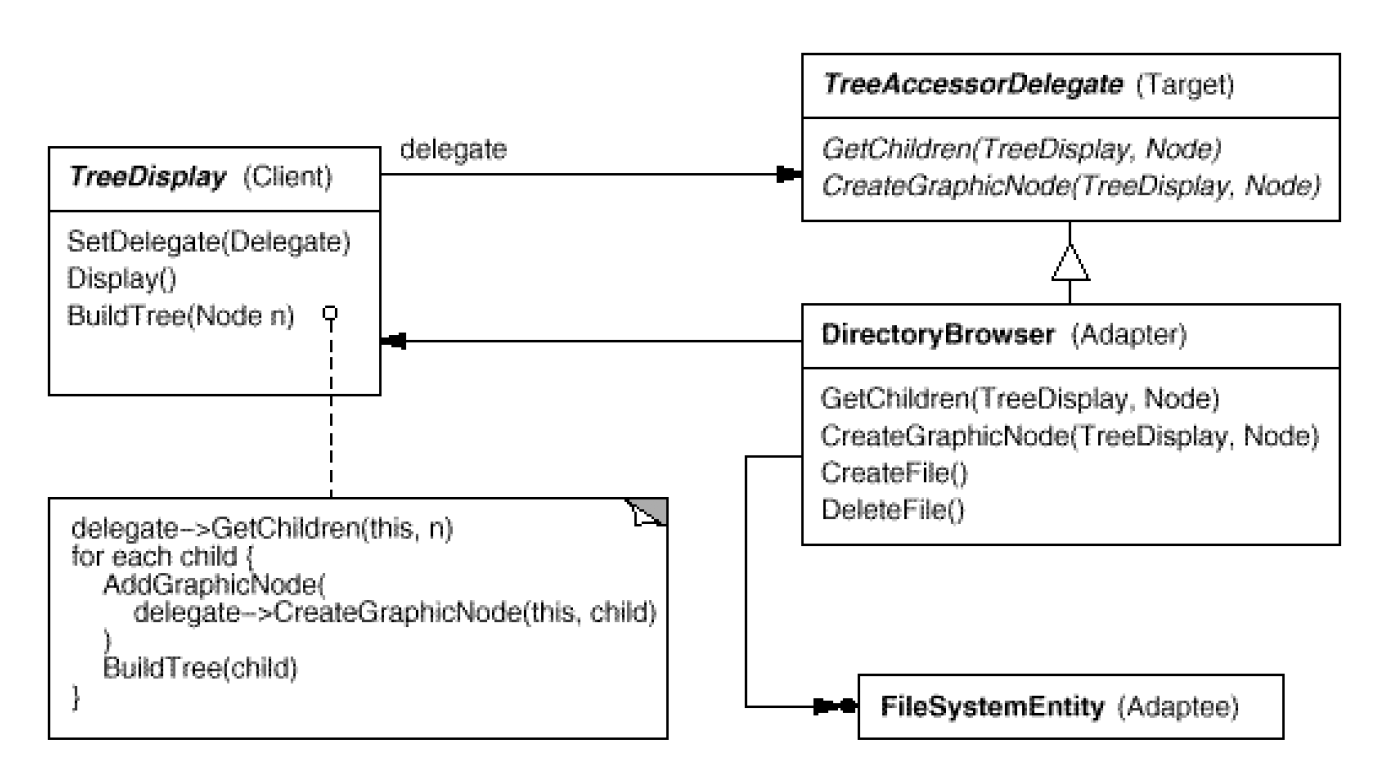
\includegraphics[scale=0.4]{pluggableadapter2.png}
\end{center}
\end{frame}
%-------------------------------------------------------------------------------------------------

\subsection{Օրինակ}
%-------------------------------------------------------------------------------------------------
\begin{frame}[fragile]\frametitle{Օրինակ}
\begin{english}
\begin{minted}[fontsize=\scriptsize]{cpp}
class Shape {

public:
    Shape();
    virtual void BoundingBox(Point& bottomLeft, Point& topRight) const;
    virtual Manipulator* CreateManipulator() const;
};

class TextView {

public:
    TextView();
    void GetOrigin(Coord& x, Coord& y) const;
    void GetExtent(Coord& width, Coord& height) const;
    virtual bool IsEmpty() const;
};
\end{minted}
\end{english}
\end{frame}
%-------------------------------------------------------------------------------------------------

%-------------------------------------------------------------------------------------------------
\begin{frame}[fragile]\frametitle{Օրինակ}
\begin{english}
\begin{minted}[fontsize=\scriptsize]{cpp}
class TextShape : public Shape, private TextView {

public:
    TextShape();
    virtual void BoundingBox(Point& bottomLeft, Point& topRight) const;
    virtual bool IsEmpty() const;
    virtual Manipulator* CreateManipulator() const;
};

void TextShape::BoundingBox(Point& bottomLeft, Point& topRight) const {

    Coord bottom, left, width, height;
    GetOrigin(bottom, left); GetExtent(width, height);

    bottomLeft = Point(bottom, left);
    topRight = Point(bottom + height, left + width);
}
\end{minted}
\end{english}
\end{frame}
%-------------------------------------------------------------------------------------------------

%-------------------------------------------------------------------------------------------------
\begin{frame}[fragile]\frametitle{Օրինակ}
\begin{english}
\begin{minted}[fontsize=\scriptsize]{cpp}
class TextShape : public Shape {

public:
    TextShape(TextView* t) : text(t) {}
    virtual void BoundingBox(Point& bottomLeft, Point& topRight) const;
    virtual bool IsEmpty() const;
    virtual Manipulator* CreateManipulator() const;

private:
    TextView* text;
};

void TextShape::BoundingBox(Point& bottomLeft, Point& topRight) const {

    Coord bottom, left, width, height;
    text->GetOrigin(bottom, left); text->GetExtent(width, height);

    bottomLeft = Point(bottom, left);
    topRight = Point(bottom + height, left + width);
}
\end{minted}
\end{english}
\end{frame}
%-------------------------------------------------------------------------------------------------

\section{Առնչվող Ձևանմուշները}
%-------------------------------------------------------------------------------------------------
\begin{frame}\frametitle{Առնչվող Նախագծման Ձևանմուշները}
\begin{itemize}
    \item Bridge \vfill
    \item Decorator \vfill
    \item Proxy
\end{itemize}
\end{frame}
%-------------------------------------------------------------------------------------------------

\end{document}
